% ==================================================
% 4.2 執行動態模型之辨識與預測驗證
% ==================================================
\section{執行動態模型之辨識與預測驗證}
\label{sec:execution_model_validation}

全身控制器需由輸入命令預測未來的底盤與手臂構型，
其中手臂的位置命令介面包含設定點累積與關節追蹤兩個過程。
本節先以自由空間運動紀錄辨識手臂追蹤模型，
再比較直接速度積分與設定點增廣模型的預測誤差，
最後分析命令生效延遲與等效偏置對狀態預測的影響。
辨識與重播計算分別沿用各組資料取得時的控制條件，
參數及誤差均對應其所屬的評估資料。

% ==================================================
% 4.2.1 手臂追蹤動態參數辨識
% ==================================================
\subsection{手臂追蹤動態參數辨識}
\label{subsec:arm_tracking_parameter_identification}

辨識資料包含六軸關節位置、實際寫入的位置設定點及物理時間戳記。
關節位置 $q_a^j$ 與設定點 $s_a^j$ 以同一物理步配對，
其中 $s_a^j$ 為作用於第 $j$ 至 $j+1$ 步的位置目標。
資料中的物理步長為 $0.01$ s，
上游控制命令每 $0.05$ s 更新，
設定點則於每一物理步依實際放行的變化率累積。
此時間關係使設定點追蹤能以第 3.2 節的逐步模型描述，
並將控制更新頻率與設定點積分頻率分別處理。

使用連續運動資料的前半段估計參數，後半段進行預測驗證。
對每個關節，以設定點與實際位置之差作為迴歸輸入，
以相鄰物理步的關節位移作為輸出，
依式\eqref{eq:ch3_arm_parameter_identification}
估計追蹤係數 $\hat\alpha_r$ 與每步偏置 $\hat b_r$。
驗證期間固定已辨識的參數，
使後續誤差反映模型對不同時間區段的預測能力。

各軸辨識結果如\cref{tab:ch4_arm_identification_parameters}所示。
為便於比較響應速度，另由離散追蹤係數換算等效時間常數：
\begin{equation}
    \tau_r=-\frac{\Delta t_p}{\ln(1-\hat\alpha_r)}.
    \label{eq:ch4_arm_equivalent_time_constant}
\end{equation}
此換算對應設定點固定時的指數衰減形式。
六軸的 $\hat\alpha_r$ 皆約為 $0.095$，
等效時間常數約為 $0.100$ s，
表示關節對設定點的追蹤會跨越數個控制週期持續進行。

\begin{table}[htbp]
    \centering
    \caption{自由空間資料之手臂追蹤動態辨識結果}
    \label{tab:ch4_arm_identification_parameters}
    \begingroup
    \small
    \renewcommand{\arraystretch}{1.2}
    \begin{tabular}{c c c c}
        \hline
        關節 & $\hat\alpha_r$ & $\hat b_r$（mrad/步） & $\tau_r$（ms） \\
        \hline
        1 & $0.095010$ & $1.194\times10^{-3}$  & $100.169$ \\
        2 & $0.095038$ & $2.715\times10^{-1}$  & $100.138$ \\
        3 & $0.095008$ & $-2.056\times10^{-2}$ & $100.171$ \\
        4 & $0.094992$ & $3.299\times10^{-3}$  & $100.189$ \\
        5 & $0.095013$ & $1.607\times10^{-4}$  & $100.166$ \\
        6 & $0.095019$ & $1.957\times10^{-5}$  & $100.159$ \\
        \hline
    \end{tabular}
    \endgroup
\end{table}

各軸的偏置量具有不同大小與方向。
以第二關節為例，設定點固定時的等效穩態偏移
$\hat b_2/\hat\alpha_2$ 約為 $2.856$ mrad；
因此，每步偏置須經追蹤動態累積後，才對應至固定設定點下的穩態差異。
在後半段資料的 $10$ ms 單物理步驗證中，
最大逐軸 RMSE 約為 $0.111$ mrad。
此結果用於描述該辨識條件下的位置介面響應，
後續再透過較長時間的預測，觀察誤差的累積情形。
控制增益、工具配置或負載改變時，
則以對應資料重新檢查參數與預測殘差。

% ==================================================
% 4.2.2 直接速度積分與增廣模型之比較
% ==================================================
\subsection{直接速度積分與增廣模型之比較}
\label{subsec:direct_augmented_model_comparison}

直接速度積分模型將設定點變化率視為關節速度，
由起始位置與區間內命令積分預測關節位置：
\begin{equation}
    \hat q_a^{\mathrm{dir}}(t+\tau\mid t)
    =q_a(t)+\int_t^{t+\tau}u_a^{\mathrm{appl}}(\lambda)\,\mathrm d\lambda.
    \label{eq:ch4_direct_velocity_prediction}
\end{equation}
離散計算時依物理步的實際命令作用區間對齊積分。
設定點增廣模型則由同一時刻的實際關節位置與設定點開始，
逐步推進設定點與關節追蹤狀態。
兩者均使用相同的驗證區段、預測起點與對應命令歷程。

首先比較一個控制週期，即 $50$ ms 的預測。
增廣模型分別採用逐步實錄設定點，
以及將整個預測區間的實際輸入平均後保持固定兩種重播方式。
前者保留區間內完整的設定點變化，
後者用於觀察輸入簡化對模型預測的影響。
兩種方式皆使用已記錄的後續輸入資訊，
評估範圍為已知輸入歷程下的離線條件預測。

\cref{tab:ch4_arm_prediction_rmse}列出與控制週期對齊之起點所得的結果。
直接速度積分的各軸 RMSE 約為 $24.988$--$25.378$ mrad，
採用實錄設定點的增廣模型則為 $0.001$--$0.444$ mrad。
改用區間平均輸入時，增廣模型的誤差為 $0.403$--$0.555$ mrad，
顯示保留設定點狀態與追蹤動態，可減少直接積分所產生的預測落差。
其中實錄設定點與區間平均輸入的差異，
亦反映控制區間內命令變化對短時預測的影響。

\begin{table}[htbp]
    \centering
    \caption{控制週期對齊之 $50$ ms 關節預測 RMSE（mrad）}
    \label{tab:ch4_arm_prediction_rmse}
    \begingroup
    \small
    \renewcommand{\arraystretch}{1.25}
    \begin{tabular}{c c c c}
        \hline
        關節 & 直接速度積分
        & \shortstack{增廣模型\\實錄設定點}
        & \shortstack{增廣模型\\區間平均輸入} \\
        \hline
        1 & $25.283$ & $0.010$ & $0.422$ \\
        2 & $25.075$ & $0.444$ & $0.555$ \\
        3 & $25.378$ & $0.035$ & $0.403$ \\
        4 & $24.988$ & $0.042$ & $0.406$ \\
        5 & $25.082$ & $0.003$ & $0.405$ \\
        6 & $25.275$ & $0.001$ & $0.417$ \\
        \hline
    \end{tabular}
    \endgroup
\end{table}

\cref{fig:ch4_arm_prediction_validation}(a)比較各軸誤差，
並以對數縱軸呈現不同量級。
為觀察預測時間增加時的變化，
另由驗證區段選取可涵蓋完整 $250$ ms 的共同起點，
分別計算 $10$、$50$、$100$、$150$ 與 $250$ ms 的預測誤差。
各時域均以實錄輸入逐步重播，
並以六軸中最大的逐軸 RMSE 作為比較量，
結果如\cref{fig:ch4_arm_prediction_validation}(b)所示。
共同起點使曲線的變化可對應至預測時間長度，
避免因評估區段不同而混入額外差異。
在 $250$ ms 時，直接速度積分與實錄設定點增廣模型的
最大逐軸 RMSE 分別約為 $102.868$ 與 $0.954$ mrad，
顯示兩者的預測差異隨評估時間延長而持續存在。

\begin{figure}[htbp]
    \centering
    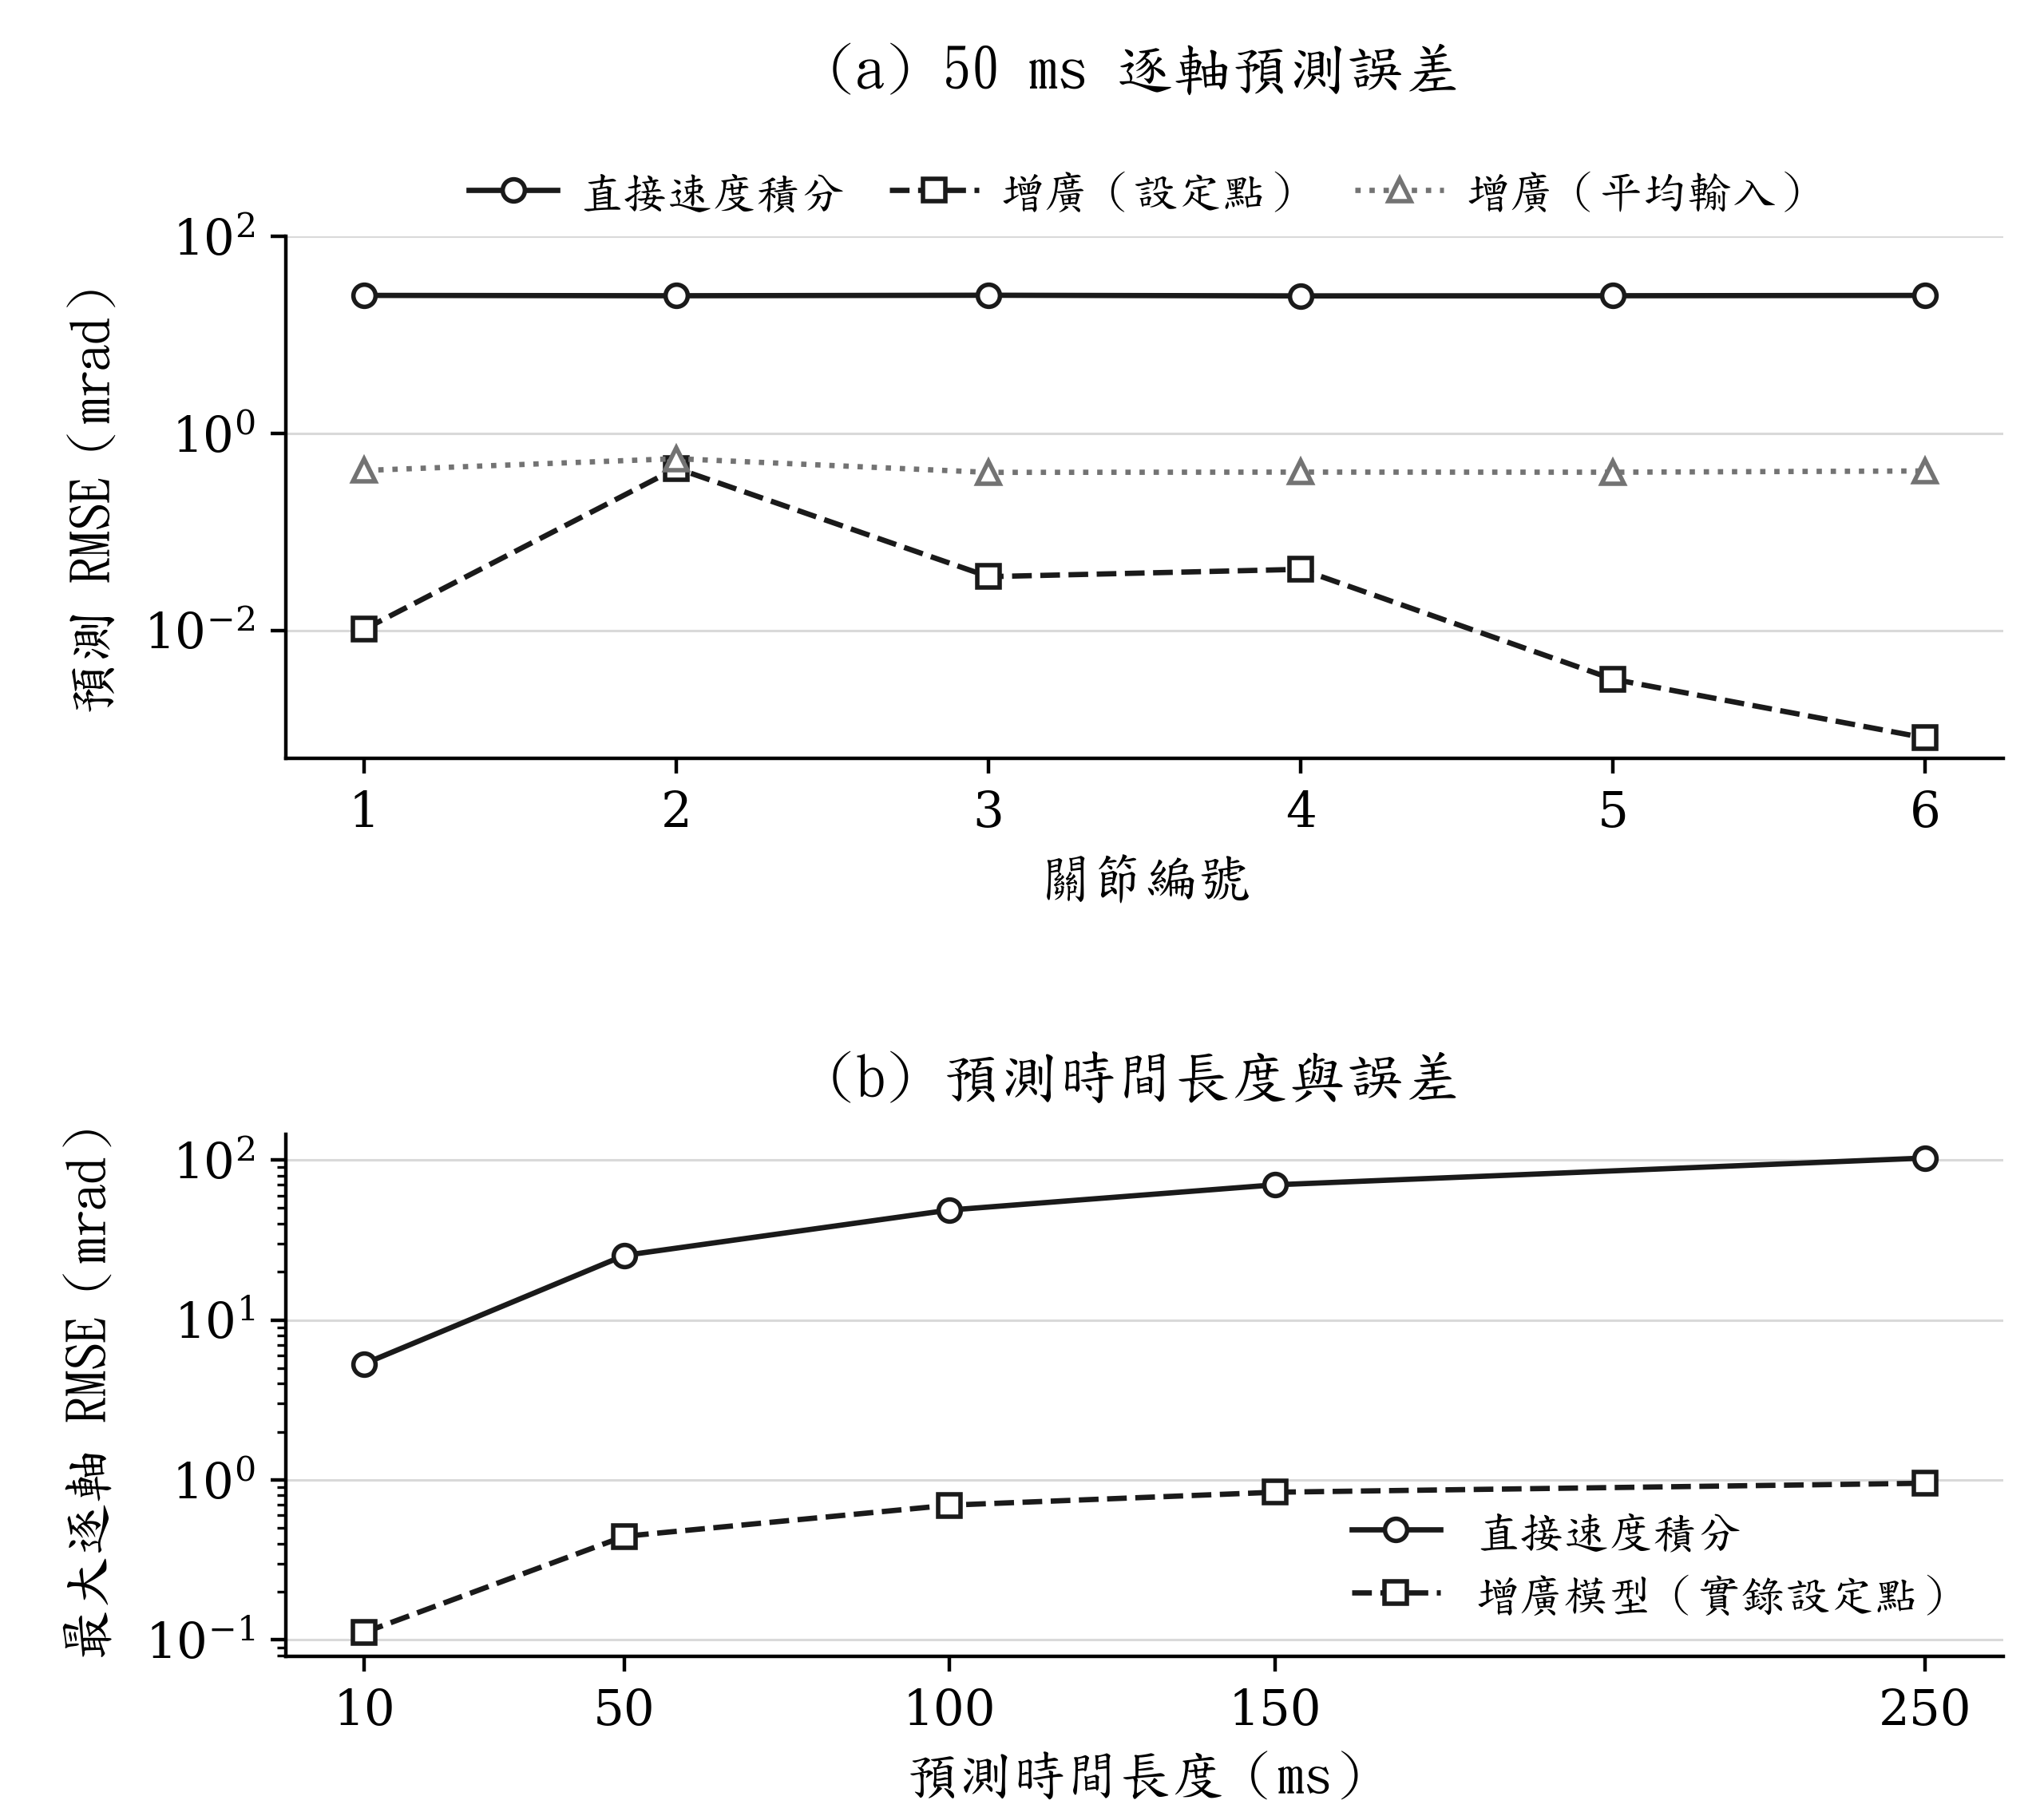
\includegraphics[width=0.98\textwidth]{figsrc/ch04/arm_model_prediction_validation.png}
    \caption{手臂執行模型之離線預測比較：
    (a) 控制週期對齊之 $50$ ms 逐軸 RMSE；
    (b) 共同起點下，不同預測時間長度的最大逐軸 RMSE。
    兩圖縱軸皆採對數尺度；區間平均輸入由該區間的實錄命令計算。}
    \label{fig:ch4_arm_prediction_validation}
\end{figure}

增廣模型能保留控制開始前已累積的設定點追蹤運動。
依本組辨識係數合成五個物理步後，
$A_q$ 與 $A_s$ 的對角元素分別約為 $0.607$ 與 $0.393$，
而設定點變化率對當期關節位置的直接係數約為 $0.00864$ s。
因此，一個控制週期內的關節位移同時取決於既有設定點差與新輸入，
其作用可由增廣狀態共同描述。
離線重播提供執行模型的預測依據，
線上控制的末端追蹤與任務表現則於後續協同操作實驗分析。

% ==================================================
% 4.2.3 命令延遲與偏置估測之影響
% ==================================================
\subsection{命令延遲與偏置估測之影響}
\label{subsec:delay_bias_effects}

模型預測除需符合關節追蹤特性，亦需對應命令實際生效時刻。
令 $t_s$ 為控制狀態的擷取時間，
$t_{\mathrm{pub}}$ 為候選命令發布時間，
$t_{\mathrm{act}}$ 為該命令首次作用於平台的時間，
狀態至生效延遲可分解為
\begin{equation}
    \tau_{\mathrm{sa}}
    =t_{\mathrm{act}}-t_s
    =(t_{\mathrm{pub}}-t_s)
     +(t_{\mathrm{act}}-t_{\mathrm{pub}}).
    \label{eq:ch4_command_activation_delay}
\end{equation}
利用 ROS 命令傳遞紀錄的來源序號，
可將求解端發布與執行端首次套用的事件逐筆配對。
自由空間紀錄中，各配置的狀態至生效延遲中位數介於 $60$--$80$ ms，
觀測到的最大值為 $140$ ms，皆以模擬時間計算。
此延遲量測對應命令傳遞時序，主機上的求解耗時另於第 4.6 節分析。

狀態取得至命令生效之間，平台仍會沿既有排程持續運動。
因此，第 3.7 節的在途命令前推保留底盤速度與設定點追蹤歷程，
再由預定生效時刻建立新一輪預測與參考。
住宅整合配置的八個物理步排程對應 $80$ ms 的預定前推長度；
實際是否能承接新控制段，仍由封包生效步及到達期限核對。
延遲分析據此區分排程等待、狀態年齡與實際生效事件，
使關節預測與參考目標使用一致的時間起點。

偏置估測則評估固定追蹤參數對持續運動的適應情形。
本項採用門扇操作紀錄，在相同實測關節軌跡與逐步設定點下，
比較固定等效偏置與區間更新兩種條件。
兩者使用相同起始偏置；區間更新的平滑時間常數為 $0.5$ s，
等效關節偏移的絕對上限為 $0.05$ rad。
每個區間均先以更新前的估計預測終點，
取得殘差後再更新偏置，
使當前區間的誤差可用於檢查先前估計的預測能力。

除逐軸關節殘差外，
另以區間起點的手臂位置雅可比，
計算殘差對 TCP 世界鉛直方向的局部投影：
\begin{equation}
    \begin{aligned}
        \rho_{q,k}
        &=q_a(t_{k+1})-\hat q_a^-(t_{k+1}),\\
        \rho_{z,k}
        &=e_z^\top\,{}^WJ_{A,p}(\chi_k)\rho_{q,k},
        \qquad e_z=\begin{bmatrix}0&0&1\end{bmatrix}^{\top}.
    \end{aligned}
    \label{eq:ch4_bias_residual_projection}
\end{equation}
其中 $\hat q_a^-$ 使用更新前的等效偏置，
$ {}^WJ_{A,p}$ 為手臂雅可比的線速度區塊。
$\rho_{z,k}$ 表示關節預測殘差對鉛直幾何位移的近似影響，
與末端目標追蹤誤差分別統計。

\cref{fig:ch4_interval_bias_residual}(a)顯示，
在此重播資料中，區間更新可降低各軸的預測殘差 RMS。
其中第二關節由約 $1.323$ 降至 $0.080$ mrad，
第三關節由約 $0.770$ 降至 $0.045$ mrad。
鉛直投影殘差的整體 RMS 則由 $0.776$ 降至 $0.045$ mm。
依門角每 $5^\circ$ 分組後，
固定偏置在較大門角區間的殘差較高，
區間更新則維持較低的殘差，
如\cref{fig:ch4_interval_bias_residual}(b)所示。
此結果支持於運動過程中，依完整追蹤區間調整等效偏置，
以維持模型對當前響應的描述能力。

\begin{figure}[htbp]
    \centering
    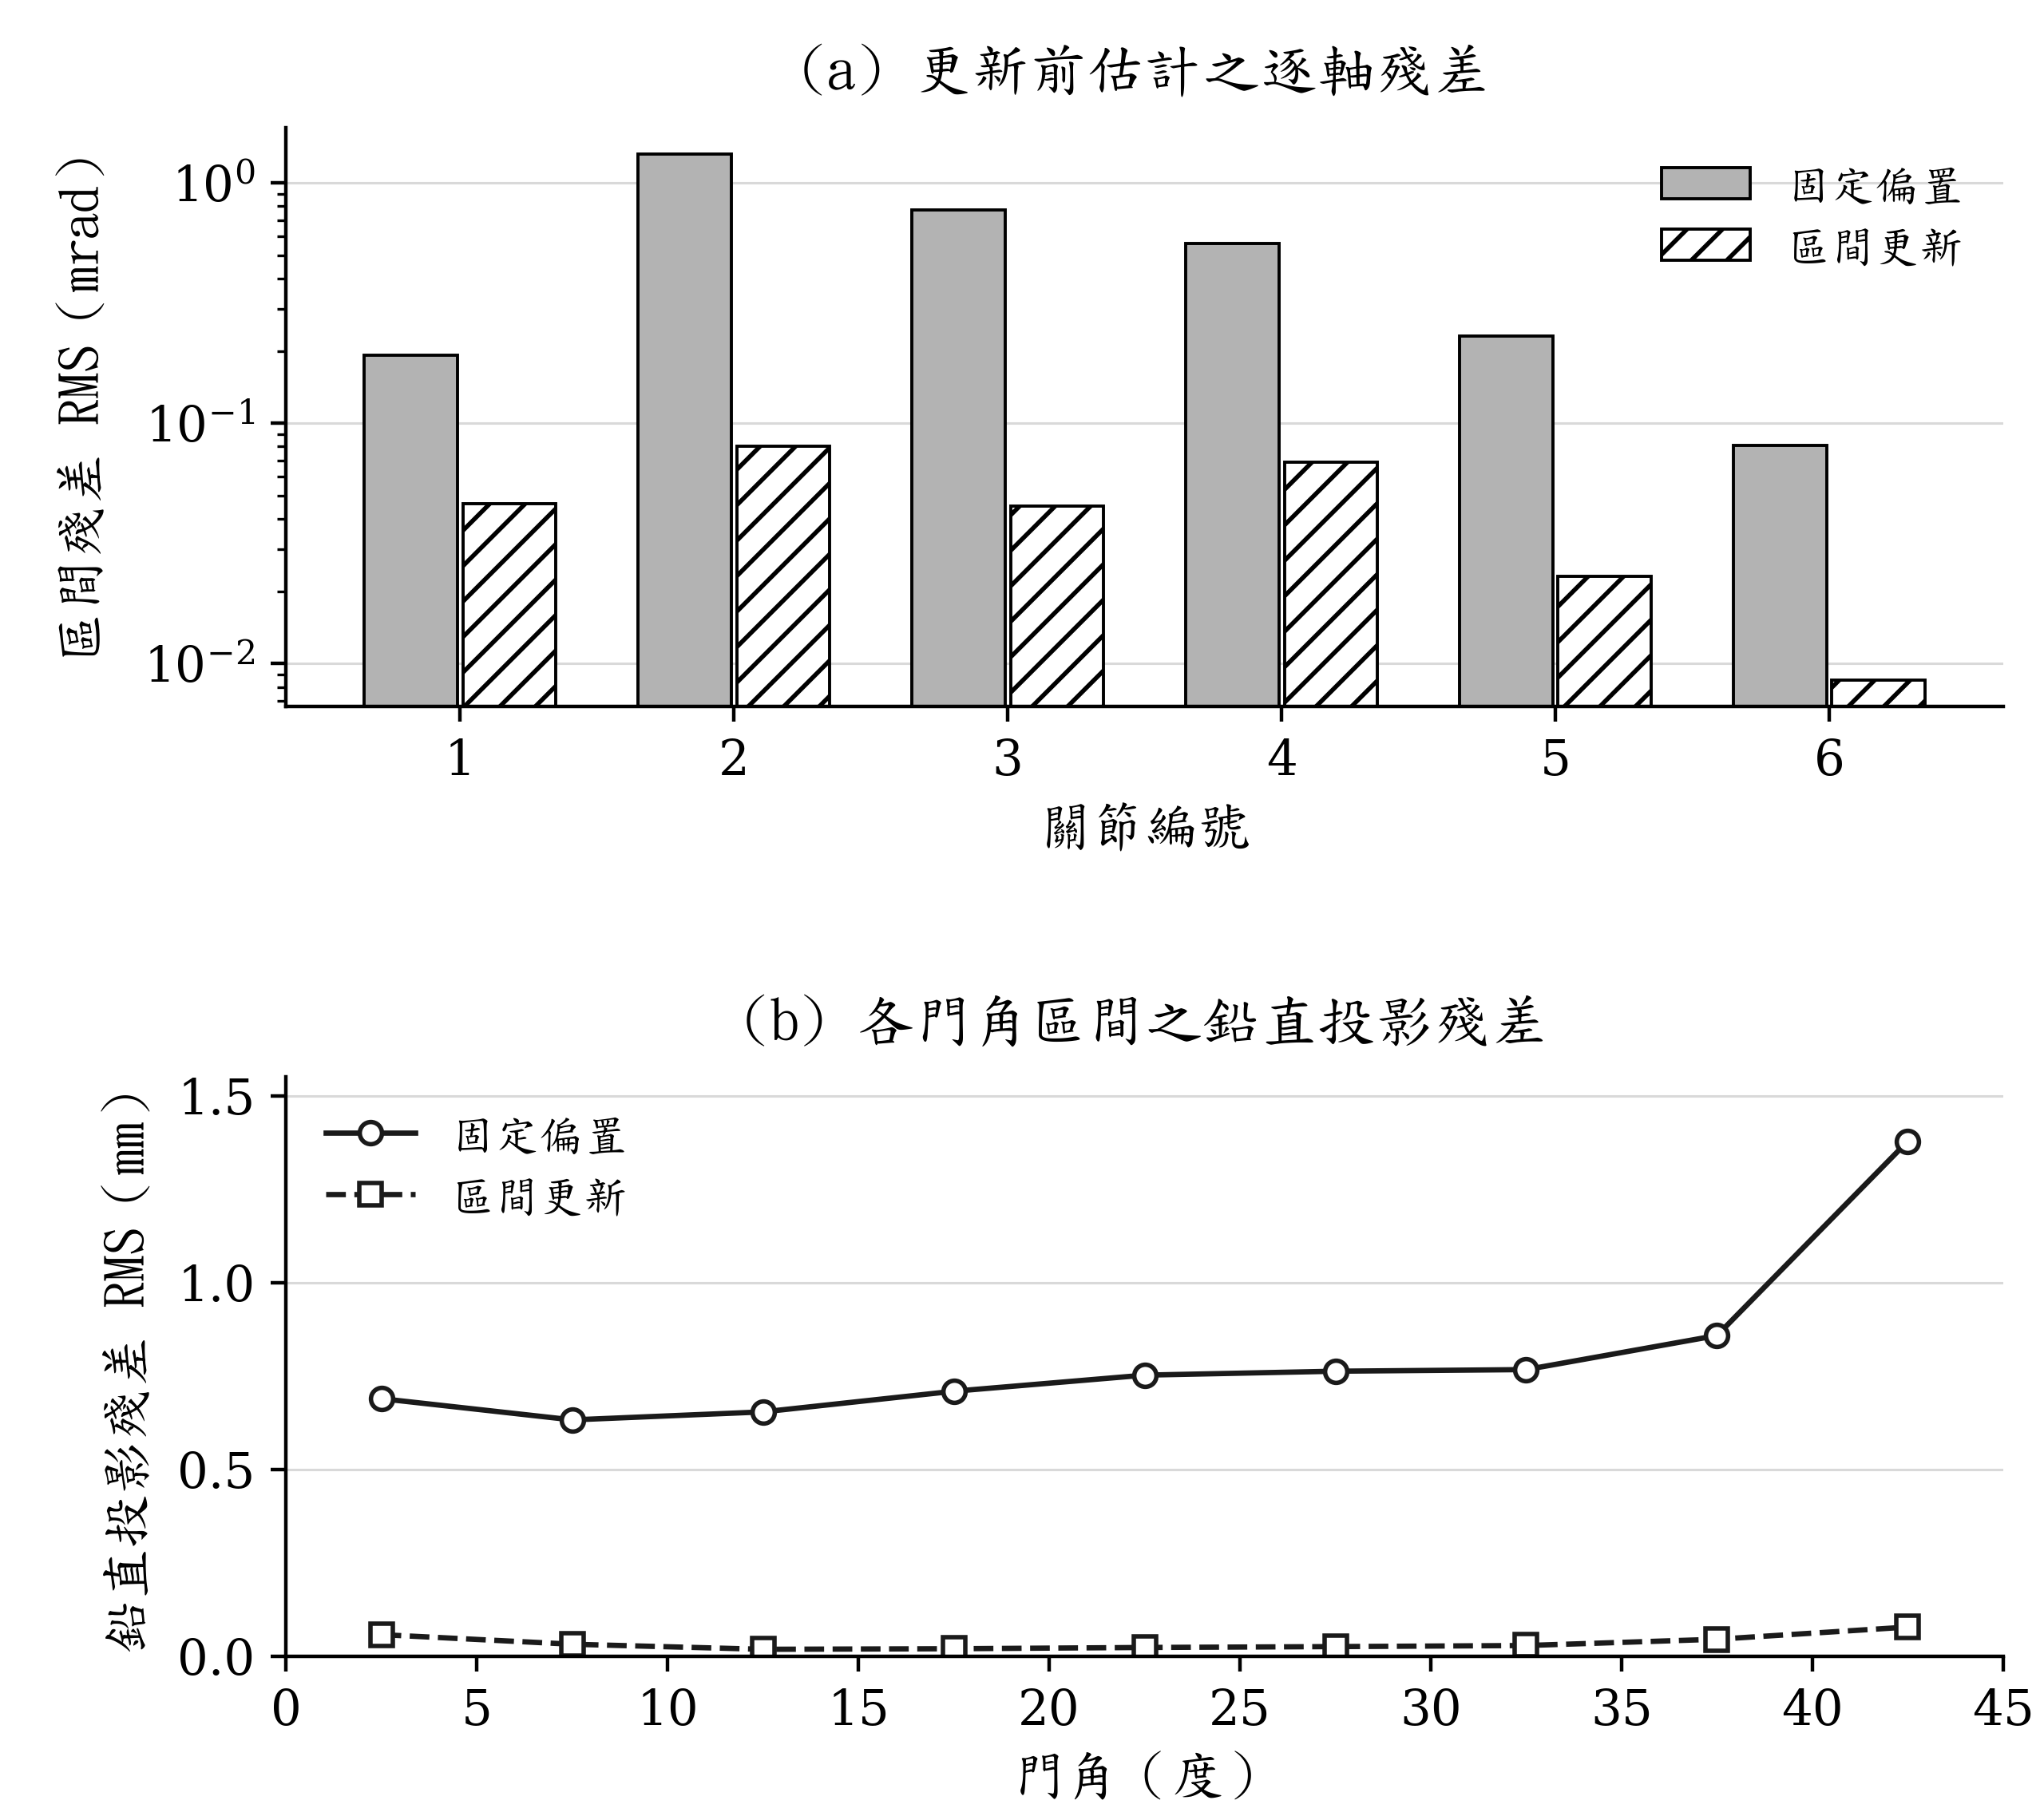
\includegraphics[width=0.98\textwidth]{figsrc/ch04/interval_bias_prediction_residual.png}
    \caption{固定偏置與區間更新之離線重播比較：
    (a) 更新前估計之逐軸區間殘差 RMS，縱軸採對數尺度；
    (b) 依門角每 $5^\circ$ 分組之鉛直投影殘差 RMS，點位於各組角度中點。
    兩條件沿用相同實測軌跡與設定點歷程。}
    \label{fig:ch4_interval_bias_residual}
\end{figure}

偏置重播的結果適用於固定實測軌跡下的區間條件預測。
等效偏移反映位置追蹤模型中的持續差異，
其物理來源可能同時包含構型、負載及未建模動態。
實際控制依任務階段設定偏置的更新與凍結條件，
並以相同參數進行 QP 預測、在途命令前推及停止檢查。
末端積分補償則維持第 3.7 節的有界目標修正方式，
其追蹤效果隨後續操作案例呈現。
